\documentclass[10pt,twoside,a4paper]{report}
\usepackage[utf8]{inputenc}
\usepackage{amsmath}
\usepackage{amsfonts}
\usepackage{amssymb}

% ETHASL package
% TODO Choose options according to your project
% som/bt/st/mt: Studies on Mechatronics, Bachelor Thesis, Semester Thesis, Master Thesis
% fs/hs: Spring term, Autumn term
% german/english: German/English
\usepackage[bt,fs,english]{packages/ethasl}

% Activate for german language
%\usepackage{german}
%\usepackage{ae}

%%%%%%%%%%%%%%%%%%%%%%%%%%%%%%%%%%%%%%%%%%%%%%%%%%%%%%%%%%%%%%%%%%%%%%%%%%%%%%%
% LaTeX preamble
%%%%%%%%%%%%%%%%%%%%%%%%%%%%%%%%%%%%%%%%%%%%%%%%%%%%%%%%%%%%%%%%%%%%%%%%%%%%%%%
% Encoding settings

% Paper size
\usepackage{a4}

% Headings
\usepackage{fancyhdr}

% More symbols
\usepackage{textcomp}\usepackage{gensymb}

% Math support for Times font
%\usepackage{txfonts}

% ISO date
\usepackage[english]{isodate}

% Multi column
\usepackage{multicol}

% Figures 
\usepackage{graphicx}

% Subfigures (obsolete)
%\usepackage{subfigure}

% Bibliography
\usepackage[numbers]{natbib}

% Clever references
\usepackage{cleveref}

% Nicer tables
\usepackage{booktabs}
\usepackage{array}
\usepackage{multirow}

% Colors
\usepackage{color}
\usepackage{colortbl}
\definecolor{black}{rgb}{0,0,0}
\definecolor{white}{rgb}{1,1,1}
\definecolor{darkred}{rgb}{0.5,0,0}
\definecolor{darkgreen}{rgb}{0,0.5,0}
\definecolor{darkblue}{rgb}{0,0,0.5}

% Additional math functionality
\usepackage{amsmath}
\usepackage{amssymb}

% Nice fractions
\usepackage{nicefrac}

% Upper case greek letters
\usepackage{upgreek}

% ISO math notation
\usepackage{isomath}
\renewcommand{\vec}{\vectorsym}
\newcommand{\mat}{\matrixsym}

% Units
\usepackage{units}

% Rotated objects
\usepackage{rotating}

% Indent
\setlength{\parindent}{0em}

% Include PDF pages
\usepackage{pdfpages}
\includepdfset{pages={-}, frame=true, pagecommand={\thispagestyle{fancy}}}

% Headings
\rhead[\thepage]{\nouppercase{\rightmark}}
\lhead[\nouppercase{\leftmark}]{\thepage}
\cfoot{}

% Links (last package)
\usepackage{url}
\usepackage{cleveref}


\title{Path Generation for a Mobile Drawing Robot}
%\subtitle{bla bla bla}

% TODO Add name of the authors
\studentA{Wolf Vollprecht}
% \studentC{Student 3}

% TODO Add name of the supervisors
\supervisionA{Nikolay Kobyshev}
\supervisionB{Philipp Krüsi}
%\supervisionC{Supervisor C}

% TODO Change if necessary
\projectYear{\the\year}
\begin{document}

\maketitle
\pagestyle{plain}
\pagenumbering{roman}

\author{Wolf Vollprecht}
\title{Path Generation for a Mobile Drawing Robot}

\begin{abstract}
The BeachBot is a mobile, autonomous drawing robot for large scale sand art. Its primary purpose is the entertainment of beachgoers. The goal of this thesis was to develop and evaluate algorithms to automatically generate suitable trajectories to draw arbitrary images on the canvas. Main challenges have been to find a trajectory that reduces the drawing time and to make watching the drawing process appealing.
\end{abstract}

\chapter{Introduction}
\section{The BeachBot Project}
The BeachBot project is a focus project at ETH Zurich. During two semesters of the bachelor studies, the team had the opportunity to develop a mobile and autonomous robot prototype for creating sand drawings on beaches (the final robot prototype is shown in \autoref{fig:beachbot}). In total 7 mechanical engineering students, one electrical engineering student and two industrial design students (from the Zürcher Hochschule der Künste) were working on the project. 

The result of the project is a three wheeled mobile robot that can drive autonomously. The key features are:
\begin{description}
\item[Localization] The robot is able to reliably localize itself on the beach, using a laser range finder and 3 or more reflective poles. The accuracy of the localization is about 3 centimetres.
\item[Driving speed and turning radius] The top speed of the robot is about 0.4 metres per second and it can turn on the spot. Both back wheels are independently steerable. The front wheel is also actuated. This is done to reduce the risk of getting stuck in sand.
\item[Rake] The main drawing tool of the robot is a rake. The rake consists of seven pin-pairs which are individually liftable.
\item[Controller] The controller uses the output from the localization to steer the robot so that it follows a pre-defined trajectory.
\item[Automatic Path Generation] An application was created to generate the trajectory for an arbitrary input drawing  that can then be drawn on the beach.
\end{description}

The robot has been successfully tested at the beach.

\begin{figure}
\centering
\begin{subfigure}[c]{1\textwidth}
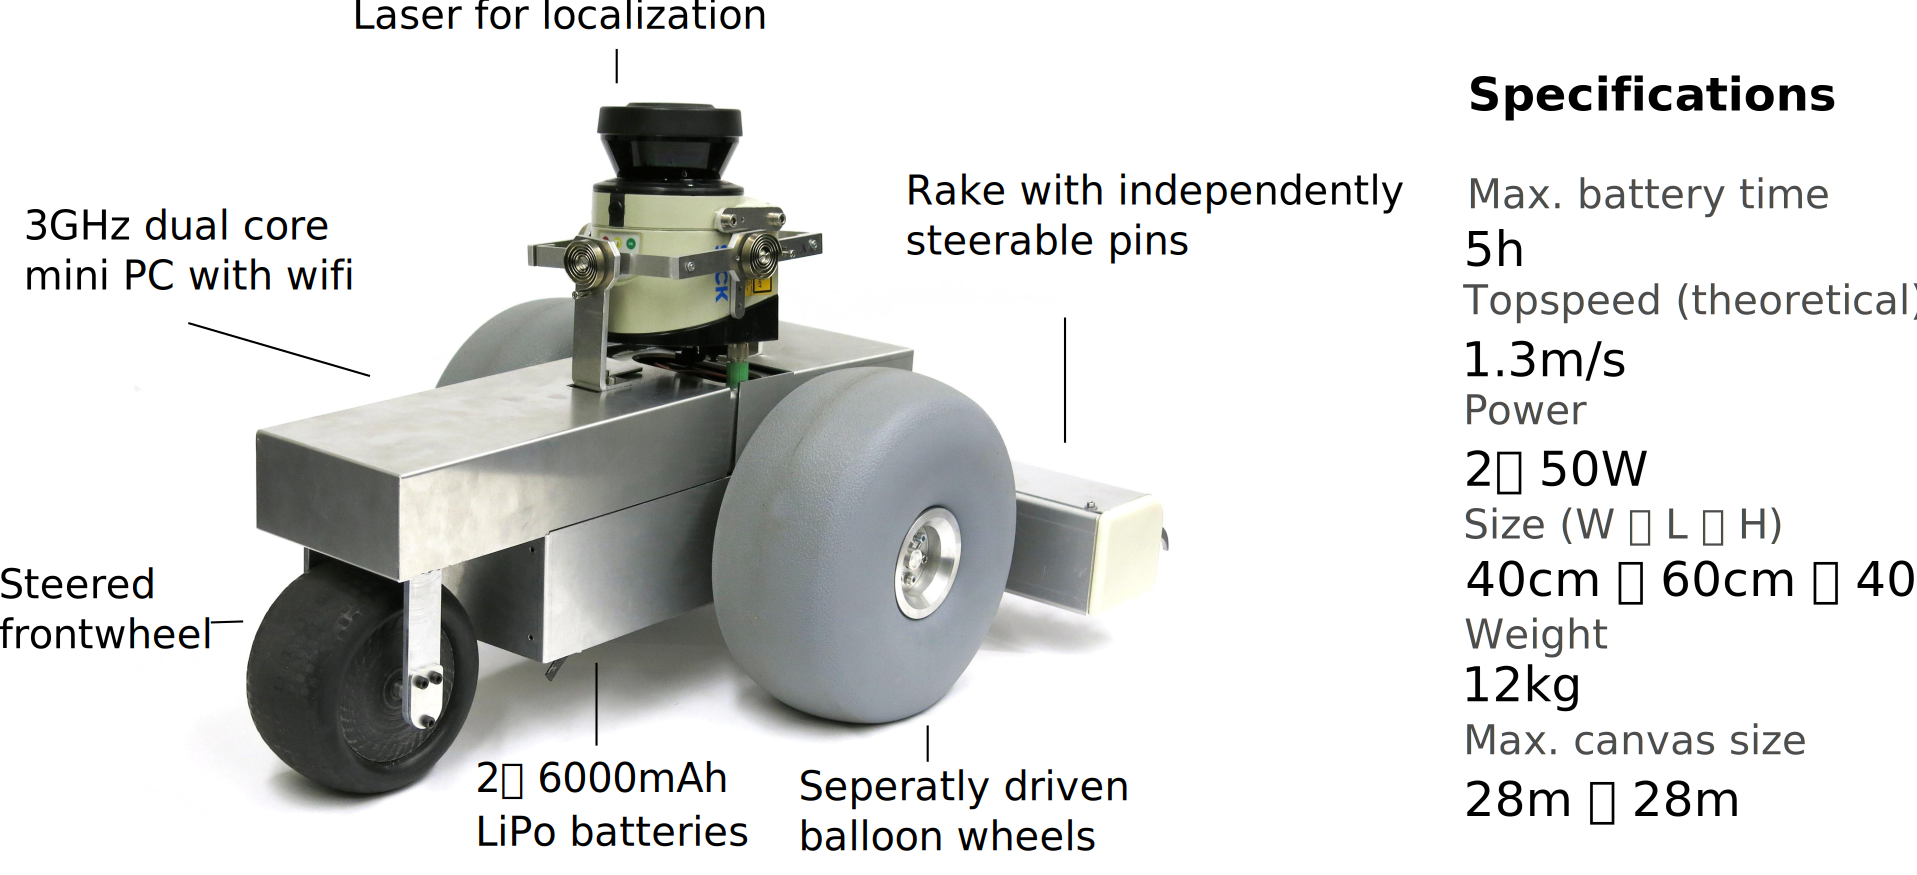
\includegraphics[width=\textwidth]{images/introduction/beachbot_spec.pdf} 
\end{subfigure}
\\
\begin{subfigure}[c]{1\textwidth}
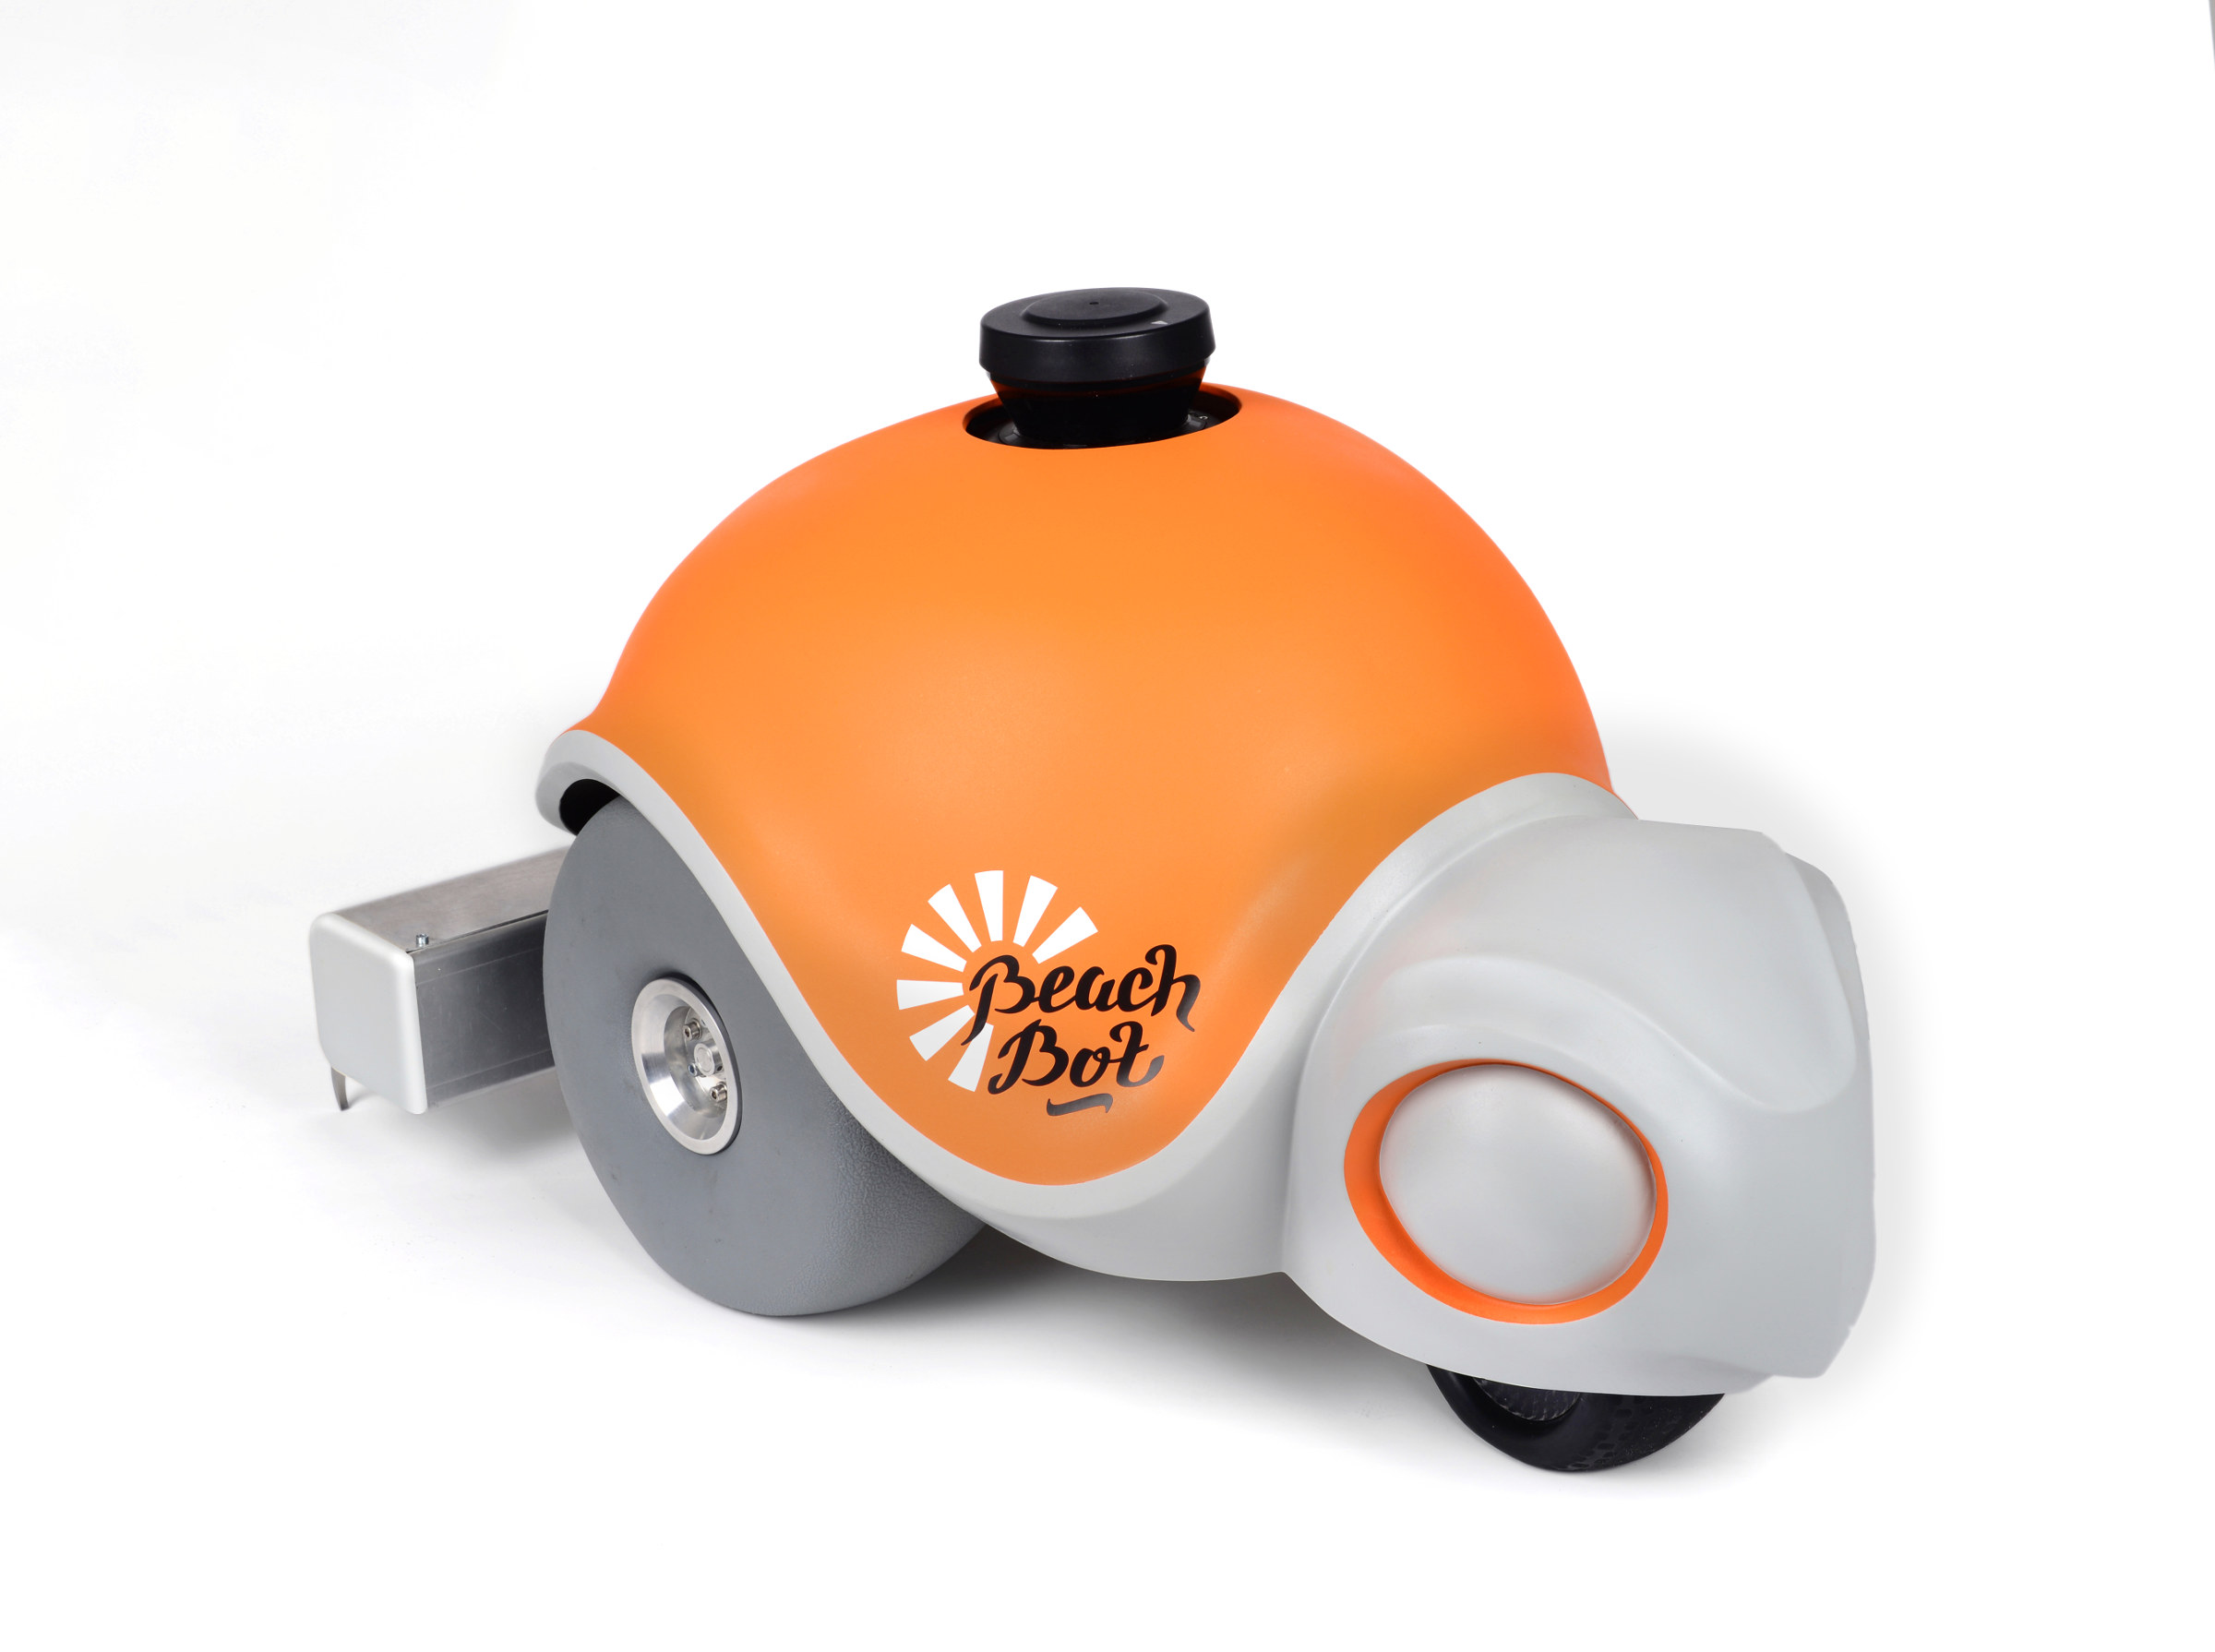
\includegraphics[width=\textwidth]{images/introduction/final_shell_scaled_down.jpg} 
\caption{The outer shell of the BeachBot}
\end{subfigure}
\\
\vspace{2cm}
\begin{subfigure}[c]{0.46\textwidth}
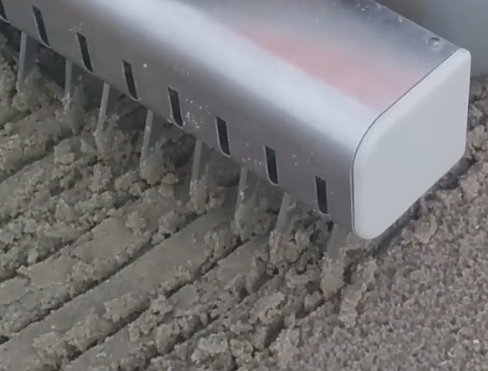
\includegraphics[width=\textwidth]{images/introduction/localization_precision.png} 
\caption{The rake in action}
\end{subfigure}
~~
\begin{subfigure}[c]{0.3\textwidth}
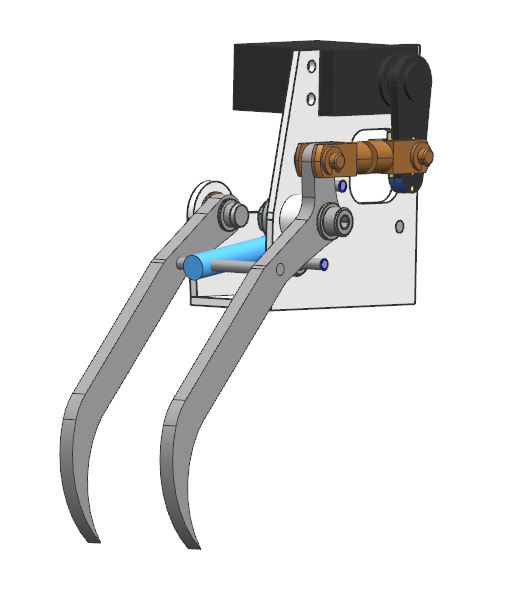
\includegraphics[width=\textwidth]{images/introduction/rake_pins.png}
\caption{One rake unit with servo motor and pin pair}
\end{subfigure}
\caption{Various images of the BeachBot}
\label{fig:beachbot}
\end{figure} 


\chapter{Requirements and Inspiration}

% here you say that the project consists of a GUI and an algorithm.

\chapter{Path planning algorithms}
\subsection{Algorithm overview}
% here you set the main requirements connected, as short as possible, no sharp angles etc)
\subsection{Image structure}%go
% you discuss the lines, closed lines, filled polygons
% then you explain the structure that you work on elements separately and the connect them with TSP.
\subsection{Polygon filling}
\subsubsection{Related work}
	% all the algorithms go here
\subsubsection{Straight Skeleton Filling}
	% your algorithm
\subsubsection{Back and Forth Filling}
	% your algorithm. \subsubsection{Optimal Convex Partitioning} goes here without a special subsection for it

\subsection{Path Generarion}
% state: we have 2 global problems
\subsubsection{Traveling Salesman Problem}
% general definition
% all three methods we tried, including LKH
\subsubsection{Adaptation of Traveling Salesman Problem for the Algorithm}
% how do you solve the problems of the closed loop in polygon and the constraint of returning to the start point

\subsection{Smooth line connections}
\subsubsection{Beziér Splines}
\subsubsection{Spiro Splines}

\section{Implementation}
\subsection{Input}	% svg files, why vector is better than raster
\subsection{SVG Parser}
\subsection{Tree Container}
\subsection{Preprocessing}
\subsection{Implementation of the Algorithms}
\subsection{Postprocessing}
\subsection{User Interface}

\chapter{Conclusion}
\end{document}
